\documentclass[aps, pre, preprint, groupedaddress, superscriptaddress, showkeys, showpacs] {revtex4-1}

\usepackage{amsmath}
\usepackage{mathtools}
\usepackage{amssymb}
\usepackage{amsfonts}
\usepackage{graphicx}
\usepackage{epstopdf}

% For the debug usage only
\usepackage{color}

\DeclarePairedDelimiter\bra{\langle}{\rvert}
\DeclarePairedDelimiter\ket{\lvert}{\rangle}

% Remove ugly line above reverences
\def\bibsection{\section*{\refname}} 

\begin{document}

\title{Quantum-Classical Phase Transition for Exciton-Polariton Josephson Junctions}

\author{A. P. Alodjanc}
\email{alexander\_ap@list.ru}
\affiliation{ITMO University, St. Petersburg 197101, Russia}

\author{M. E. Lebedev}
\email{m.lebedev@lmc.ifmo.ru}
\affiliation{ITMO University, St. Petersburg 197101, Russia}

\date{\today}

\begin{abstract}
Abstract will be placed here.
\end{abstract}

\pacs{\dots}
\keywords{\dots}

\maketitle

\newcommand{\sn}{\textrm{sn}}
\newcommand{\cn}{\textrm{cn}}
\newcommand{\dn}{\textrm{dn}}
\newcommand{\sd}{\textrm{sd}}
\newcommand{\cd}{\textrm{cd}}
\newcommand{\nd}{\textrm{nd}}
\newcommand{\am}{\textrm{am}}

% For the debug usage only
\newcommand{\red}{\color{red}}

\section{Introduction \label{sec:introduction}}

For last decade investigations of exciton polariton Bose-Einstein condensates (BEC) in various type of semiconductor microstructures represent one of mainstreams of current photonic and semiconductor technologies, see e.g. \cite{1,2}.
The microcavity exciton polaritons are bosonic quasiparticles representing  admixtures of the quantized cavity mode and quantum wells excitons.
Practically, semiconductor microcavities are promising for various optoelectronic applications where quantum  matter-field interface plays crucial role.
In particular, demonstrations of polariton laser with electrical pump \cite{3,4}, amplifiers \cite{5}, switches \cite{6}, transistors \cite{7}, polariton circuits and optical logic elements \cite{8,9}.
Although exciton polariton condensates exhibits Bose-Einstein statistics under the phase transition condition and macroscopic occupation of the ground state at certain pumping rate that is less than for convenient lasers, they are not in true thermodynamic equilibrium state \cite{10,11}.
  
Non-equilibrium, or, thermodynamically quasi-equilibrium features of exciton polariton condensates play certain role in various manifestations of their collective (many body) quantum states such as superfluidity \cite{12,13}, quantized vortices \cite{14,15}, soliton formation \cite{16}, Josephson oscillations and macroscopic self-trapping \cite{17,18}.
Since exciton polariton BEC's in present experiments examined at high enough (up to the room) temperatures the quantum character of such a states should be examined even at equilibrium.

The problem of distinguishability of statistically classical and quantum regimes for exciton polariton condensates behavior is very actual for practical purposes, see e.g. \cite{19}; especially for their possible applications for quantum information science purposes.
Fast switching properties (the typical switching time of a few picoseconds), relatively strong nonlinear response and flexibility to external optical and/or electrical pump, spin degrees of freedom made microcavity polaritons potentially very promising for quantum computation and quantum information processing objectives, see, e.g. \cite{21,22,23}. In particular, we would like to mention here problems of design ultrafast quantum gates \cite{22,23}, creation of relatively long Rabi oscillations \cite{19, 20} and quantum annealing problem \cite{24} where collective (bosonic) character of polariton BEC could be used.
Another promising area of potential applications of quantum exciton polariton states is connected with quantum metrology for which designing of quantum interferometers and gyroscopes possessing high precision measurements with quantum phase states is utilized, cf. \cite{25, 26}.
  
In the paper we consider generic problem of quantum-classical phase transition with exciton polariton condensates occurring in semiconductor microcavity in the presence of Josephson effect with them, cf. \cite{27}.
In general this area of research is based on dissipative tunneling problem or, tunneling at certain temperatures models, cf. \cite{28,29,30}.
Evidently seminal studies on this topic relay to superconductor devices \cite{31} where macroscopic tunneling plays essential role.
In particular, it worth to mention here Schr\"odinger cat state formation \cite{32} and design of quantum gates for quantum computing with superconductor qubits where macroscopic quantum coherent phase properties are used \cite{33}.
Latterly the problem of quantum tunneling and quantum-classical phase transition problem have been applied to other two-level (spin) systems, like atomic BEC's \cite{34}, and small ferromagnetic particles, \cite{35}.
Strictly speaking main discussion is focused on investigation of quantum-classical escape rate transition that takes place in the presence of potential barrier at finite temperatures.
  
In the paper we propose \textit{extended model} for exciton polariton Josephson junctions when energy of polariton-polariton scattering contributes into the tunneling parameter, cf. \cite{36,37,38} and references therein.
In particularly, we pay our attention to temperature dependent critical phenomena occurring in the presence of macroscopic tunneling.
We aimed at elucidation of necessary criteria to obtain quantum phase regimes with trapped exciton polaritons suitable for creation of exciton polariton qubit gates.

This paper is arranged as follows.
In Sec. \ref{sec:model} we explain in details our model to realize Josephson junction with exciton polariton condensates.
The extended tight-binding model will be established in this case. In Sec. \ref{sec:quantum_phase} we \dots.
In the conclusion, we summarize the results obtained.

\section{THE MODEL OD EXCITON POLARITON JOSEPHSON JUNCTION \label{sec:model}}

We start by describing the problem of equilibrium exciton polariton condensate trapping in symmetric one dimensional double well potential $U(x) = h ((x/x_0)^2 - 1)^2$, sketched on the Fig. \ref{pic:potential_sym_asym}; $2x_0$ defines distance between potential minima, $h$ depth of the potential.
% 
\begin{figure}[ht]
\center{\includegraphics[width=0.65\linewidth]{pic/potential_sym_asym.png}}
\caption{
Confined double-well potential for exciton polariton coupled condensate channels with symmetric $(\Phi_+(x))$ and asymmetric $(\Phi_-(x))$ wavefunctions obtained numerically by solving stationary GPE (\ref{eq:stationary}).
The dimensionless parameters for the calculations are: $h = 10$, $x_0 = 1$, $\mu_+ = 5.7355$, $\mu_- = 6.5653$.
\label{pic:potential_sym_asym}
}
\end{figure}
%
The Hamiltonian for the system of weakly interacting exciton polaritons in an external $U(x)$ can be written in the second quantized form as:
%
\begin{equation}
\hat{H} = \int \Big\{ -\dfrac{1}{2} \hat{\psi}^\dag \dfrac{d^2 \hat{\psi}}{dx^2} + \hat{\psi}^\dag \hat{\psi} U(x) + \dfrac{g}{2} \hat{\psi}^{\dag 2} \hat{\psi}^2  \Big\} dx,
\label{eq:gpe_hamiltonian}
\end{equation}
%
where $\hat{\psi} \equiv \hat{\psi}(x, t)$ is a polariton field operator that annihilate a particle at the position $x$ and time $t$, $g$ is two-body (polariton-polariton) scattering length.
In the paper we use so-called two-mode representation of $\hat{\psi}$ supposing
%
\begin{equation}
\hat{\psi} = \hat{\psi}_1(t) \Phi_1(x) + \hat{\psi}_2(t) \Phi_2(x),
\label{eq:two_modes}
\end{equation}
%
where $\hat{\psi}_{1,2}$ are time dependent operators characterizing condensate at the left and at the right wells respectively; $\Phi_{1,2}(x)$ are condensate wavefunctions which are responsible for it spatial distribution.
It's instructive to recast $\Phi_{1,2}(x)$ as
%
\begin{equation}
\Phi_{1,2} = \dfrac{\Phi_+ \pm \Phi_-}{\sqrt{2}}
\label{eq:basic_modes}
\end{equation}
%
where $\Phi_{\pm}(x) = \pm \Phi_{\pm}(-x)$ are symmetric $\Phi_+$ and antisymmetric $\Phi_-$ real wavefunctions obeying stationary Gross-Pitaevskii equations, respectively
%
\begin{equation}
\mu_{\pm} \Phi_{\pm} = -\dfrac{1}{2} \dfrac{d^2 \Phi_{\pm}}{dx^2} + U(x) \Phi_{\pm} + g \Phi_{\pm}^3.
\label{eq:stationary}
\end{equation}
%
and normalization condition $\int \Phi_{\pm}^2 dx = 1$.
Here $\mu_{\pm}$ are chemical potentials.
As a result an operator $\hat{\psi_1}^\dag\hat{\psi_1} + \hat{\psi_2}^\dag\hat{\psi_2} = N$ characterizes total number of particles (here and thereafter we omit ``hat'' design for simplicity).
Substituting (\ref{eq:basic_modes}), (\ref{eq:two_modes}) into (\ref{eq:gpe_hamiltonian}) we arrive to
% 
\begin{equation}
\begin{array}{lcl}
\hat{H} & = & \dfrac{A}{2} (\hat{\psi}_1^{\dag 2} \hat{\psi}_1^2 + \hat{\psi}_2^{\dag 2} \hat{\psi}_2^2) - \dfrac{G}{2} (\hat{\psi}_1^\dag \hat{\psi}_2 + \hat{\psi}_1 \hat{\psi}_2^\dag) \\ [8pt]
& & -\dfrac{\Gamma}{2} (\hat{\psi}_1^{\dag 2} \hat{\psi}_1 \hat{\psi}_2 + \hat{\psi}_1^\dag \hat{\psi}_1^2 \hat{\psi}_2^\dag + \hat{\psi}_1^\dag \hat{\psi}_2^\dag \hat{\psi}_2^2 + \hat{\psi}_1 \hat{\psi}_2^{\dag 2} \hat{\psi}_2) \\ [8pt]
& & +\dfrac{C}{2} (\hat{\psi}_1^{\dag 2} \hat{\psi}_2^2 + 4 \hat{\psi}_1^\dag \hat{\psi}_1 \hat{\psi}_2^\dag \hat{\psi}_2 + \hat{\psi}_1^2 \hat{\psi}_2^{\dag 2}),
\end{array}
\label{eq:hamiltonian}
\end{equation}
%
where we made some denotations
%
\begin{equation}
\begin{array}{c}
\gamma_{ij} = g \int \Phi_i^2 \Phi_j^2 dx, \quad i,j \in \{+,-\}; \\
\quad A = \dfrac{\gamma_{++} + \gamma_{--} + 6 \gamma_{+-}}{4}; \quad \Gamma = \dfrac{\gamma_{++} - \gamma_{--}}{2}; \\
C = \dfrac{\gamma_{++} + \gamma_{--} - 2\gamma_{+-}}{4}; \\
G = \mu_- - \mu_+ - 2\Gamma.
\end{array}
\label{eq:subs}
\end{equation}
%

Hamiltonian (\ref{eq:hamiltonian}) represents extended model for internal Josephson junction effect with exciton polariton BEC trapped in double well potential.
It is implies existence of quantum tunneling of the particles between wells with effective (nonlinear) tunneling rate
%
\begin{equation}
G_{eff} = \dfrac{1}{2}(G+\Gamma N - C\hat{\psi}_1^\dag\hat{\psi}_2).
\label{eq:tunneling_rate}
\end{equation}
%
The contribution from relevant coefficients on can be estimated from variational ansatz
%
\begin{equation}
\Phi_{\pm} = A_{\pm} \Big[ \exp \Big( -\dfrac{(x - x_0)^2}{2 a^2} \Big) \pm \exp \Big( -\dfrac{(x + x_0)^2}{2 a^2} \Big) \Big]
\label{eq:two_modes_eq}
\end{equation}
%
where $a$ is width of condensate wavefunctions at each wells (we suppose them equal to each other), defined from normalization conditions.
In Fig. \ref{pic:gamma_pm_vs_g} the behavior of normalized coefficients $\dfrac{\gamma_{ij}}{g}$ $i,j \in \{+,-\}$ as a function of half of intra-well distance $x_0$ is shown.
It is important that at differences between them rapidly vanishes with increasing of distance $x_0$.
We can suppose $\Gamma = C = 0$ for $x_0 >> a$.
This limit exactly corresponds to familiar problem of two weakly linked condensates at zero temperature \underline{- see e.g. ~\cite{39} and cf. }.
%
\begin{figure}[ht]
\center{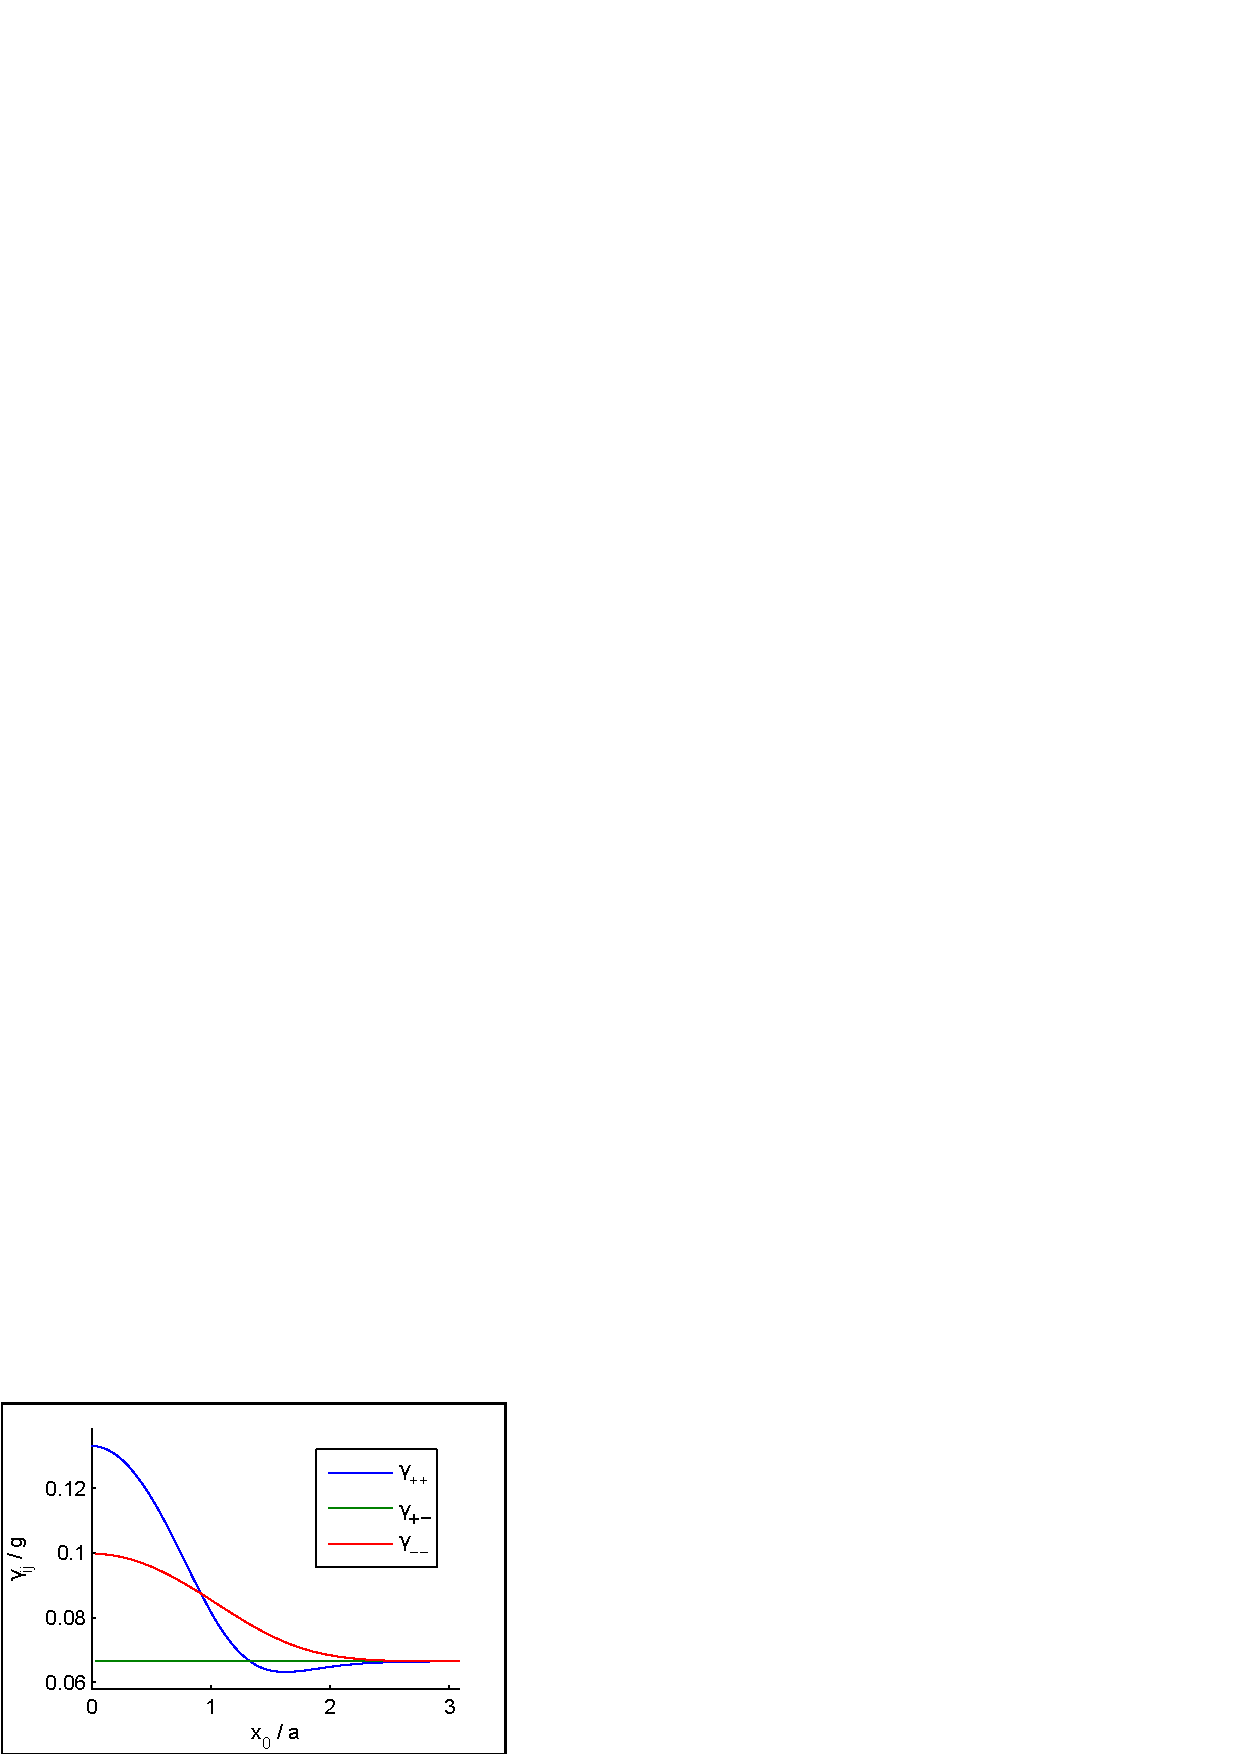
\includegraphics[width=0.65\linewidth]{pic/ypm_x0.png}}
\caption{Dependence of $\gamma_{ij} / g$ versus $x_0 / a$ \label{pic:gamma_pm_vs_g}}
\end{figure}
%

\section{The Quantum Phase \label{sec:quantum_phase}}

To elucidate important quantum phase features of our extended Josephson model it is fruitful to recast Hamiltonian (\ref{eq:hamiltonian}) through the pseudo-spin operators defined as
% 
\begin{subequations}
\begin{align}
\hat{S}_x = \dfrac{1}{2} (\hat{\psi}_1^\dag \hat{\psi}_2 + \hat{\psi}_1 \hat{\psi}_2^\dag) = s \cos(\phi) - \sin(\phi) \dfrac{d}{d \phi}, \\
\quad \hat{S}_y = \dfrac{i}{2} (\hat{\psi}_1^\dag \hat{\psi}_2 - \hat{\psi}_1 \hat{\psi}_2^\dag) = s \sin(\phi) + \cos(\phi) \dfrac{d}{d \phi}, \\
\hat{S}_z = \dfrac{1}{2} (\hat{\psi}_2^\dag \hat{\psi}_2 + \hat{\psi}_1^\dag \hat{\psi}_1) = -i\dfrac{d}{d \phi},
\end{align}
\label{eq:pseudo_spin}
\end{subequations}
%
where $s = \dfrac{N}{2} >> 1$ is large {\red $C$ - number}, $\phi$ is phase variable.
The operators determined in Eq. (\ref{eq:pseudo_spin}) obey familiar $SU(2)$ algebra commutation relations
%
\begin{equation}
[S_x, S_y] = iS_z, \quad[S_z, S_x] = iS_y, \quad[S_y, S_z] = iS_x.
\label{eq:commutation_relations}
\end{equation}
%
After straitforward calculations from (\ref{eq:hamiltonian}) one can obtain
%
\begin{equation}
\begin{array}{lcl}
H & = & -(\alpha - \beta \sin^2 \phi) \dfrac{d^2}{d \phi^2} - (\beta(s-\dfrac{1}{2})\sin{2\phi} - B\sin{\phi}) \dfrac{d}{d \phi} \\
&& - Bs \cos \phi - \beta s^2 \sin^2 \phi - \beta s \cos^2 \phi.
\end{array}
\label{eq:hamiltinian_s}
\end{equation}
%
where $\alpha = A - C = 2\gamma_{\pm} > 0$, $\beta = 2C > 0$ and $B = \Gamma N + G > 0$.
Below we chose $x_0$ obeying to condition $\gamma_{++} \simeq \gamma_{--} = \gamma$ supposing $\Gamma = 0$ for simplicity, see Fig. \ref{pic:gamma_pm_vs_g}

Hamiltonian (\ref{eq:hamiltinian_s}) corresponds to Schrodinger equation
%
\begin{equation}
\begin{array}{l}
(\alpha - \beta \sin^2 \phi) \dfrac{d^2 \Phi}{d \phi^2} + (\beta(s - \dfrac{1}{2})\sin{2\phi}-B\sin{\phi})) \dfrac{d \Phi}{d \phi} \\
+ (E + BS \cos \phi + \beta S^2 \sin^2 \phi + \beta S \cos^2 \phi) = 0.
\end{array}
\label{eq:schrodinger}
\end{equation}
%
where $\Phi \equiv \Phi(\phi)$ is unknown $2\pi$-periodic wavefunction that characterizes quantum phase properties, cf. \cite{40}.
Noticing that Eqs. (\ref{eq:hamiltinian_s}), (\ref{eq:schrodinger}) can be obtained by applying so-called phase-state representation, {\red cf. [  ]}.
%
\begin{equation}
\ket{\psi} = \dfrac{1}{2 \pi} \int_{-\infty}^{+\infty} d \phi \Phi(\phi) \ket{\phi}
\end{equation}
%
where
%
\begin{equation}
\ket{\phi} = \dfrac{1}{\sqrt{N!}} \Big[ e^{i\phi/2} \psi_1^\dagger + e^{-i \phi/2} \psi_2^\dag \Big]^N \ket{0}_1\ket{0}
\end{equation}
%
is macroscopic coherent spin-state (macroscopic qubit state) that plays important role in current quantum information protocols operating with $N$-particle condensates, cf. \cite{41}.
It is possible to eliminate the term with first derivative in Eq.(\ref{eq:schrodinger}) applying the transformation
%
\begin{equation}
\Phi(\phi) = \Psi(z) \exp \Big( s \log \dn{z} - \dfrac{\Lambda s}{2 \sqrt{\lambda (1 - \lambda)}} \arctan \Big( \sqrt{\dfrac{\lambda}{1 - \lambda}} \cn{z} \Big) \Big)
\label{eq:transformation_of_phi}
\end{equation}
%
where
%
\begin{equation}
z = \int \limits_0^\phi \dfrac{d \xi}{\sqrt{1 - \lambda \sin^2 \xi}} = F(\phi, \sqrt{\lambda})
\end{equation}
is new phase variable; $F(\phi, \sqrt{\lambda})$ is incomplete elliptic integral of the first kind.
In (\ref{eq:transformation_of_phi}) we have introduced dimension-less vital parameters $\Lambda = \dfrac{G}{\alpha s}$, $\lambda = \dfrac{\beta}{\alpha}$ completely characterizing our model.

Inserting (\ref{eq:transformation_of_phi}) into (\ref{eq:schrodinger}) we come to convenient Schr\"odinger equation
%
\begin{equation}
\dfrac{d^2\Psi}{dx^2} + (E - V(x))\Psi = 0
\label{eq:schrodinger_usual}
\end{equation}
%
for quantum particle with mass $m_{eff} = \dfrac{1}{2}$, normalized energy $E \equiv \dfrac{E}{\alpha}$ moving in the potential $V(x) = s^2 V_0(x)$ with
%
\begin{equation}
V_0(x) = \frac{ (\frac{1}{4} \Lambda^2 - \lambda (1 - \lambda)) \sn^2{x} - \Lambda \cn{x}}{\dn^2{x}}
\label{eq:potential}
\end{equation}
%

The results known for quantum phase mesoscopic Josephson junction model can be recovered from (\ref{eq:schrodinger_usual}), (\ref{eq:potential}) at $\lambda = 0$.
The dependence of the $\lambda$ parameter on normalized half of intra-well distance $\dfrac{x_0}{a}$ can be estimated from (\ref{eq:subs}), (\ref{eq:two_modes_eq}) and reads as $\lambda = 0.5 \Big( \exp \Big[ \dfrac{2 x_0^2}{a^2} \Big] - 1 \Big)^{-1}$.
The limit $\lambda = 0$ obtained for infinitely large intra-well distances $x_0 \to \infty$.
On the other hand, parameter grows rapidly at $\dfrac{x_0}{a} \ll 1$.
Obviously, in this limit our Josephson junction model inherent based on relatively weak coupling between wells breaks down.
Below we examine case of $0 < \lambda < 1$ that could be obtained at moderate values $\dfrac{x_0}{a}$ of such as $\dfrac{x_0}{a} \geq 0.45$. 

Analysis of the quantum phase for exciton polariton junctions we examine in three domains of  governed parameter $\Lambda$, cf. \cite{40}.
The dependences of trapping potential $V_0(x)$ are shown in Fig. \ref{phase_potential}.
The period of the functions is determined as $4K(\lambda)$.
%
\begin{figure}[ht]
\begin{minipage}[htbp]{0.32\linewidth}	{\includegraphics[width=1\linewidth]{pic/potential_L=100.png} \\ a}
\end{minipage}
\begin{minipage}[htbp]{0.32\linewidth}	{\includegraphics[width=1\linewidth]{pic/potential_L=05.png} \\ b}
\end{minipage}
\begin{minipage}[htbp]{0.32\linewidth}	{\includegraphics[width=1\linewidth]{pic/potential_L=001.png} \\ c}
\end{minipage}
\caption{
Effective potential $V_0(z)$ for (a) $\Lambda = 100$, (b) $\Lambda = 0.5$ , and (c) $\Lambda = 0.01$ as a function of  elliptic integral phase coordinate $z$.
Points $A, B$ and $C$ in (b) corresponds to minima of the potential occurring with periodicity $4K(\lambda)$. \label{phase_potential}}
\end{figure}
%

\subsection{Rabi regime}

Here we suppose that $\Lambda \gg 1$.
In this limit the trapping potential reads
%
\begin{equation}
V_R(z) = \dfrac{1}{4} \Lambda^2 \sd^2{z}
\label{eq:rabi_potential}
\end{equation}
%
It is interesting to note that even in this case the role of $\lambda$-parameter is evident --- see Fig. \ref{phase_potential}a.

\subsection{Fock regime}

In purely quantum limit the two mode system approaches by the state $\ket{\psi} \propto (\psi_1^\dag)^s (\psi_1^\dag)^s \ket{0}_1 \ket{0}_2$ with limiting value of the phase wavefunction $\Phi(\phi) \to (2\pi)^{-1/2}$.
In this regime we distinguish two limits.
First, we suppose that inequality $\Lambda \ll \lambda \ll 1$ is holds.
In this case from (\ref{eq:potential}) one can obtain
%
\begin{equation}
V_F(z) = -\lambda(1 - \lambda) \sd^2{z}
\label{eq:fock1_potential}
\end{equation}.
%

{\red Mathieu equaiton and it's spectrum}

Another limit that could be studied within Fock regime is relevant to condition $\lambda \ll \Lambda \ll 1$.
In this case from (\ref{eq:potential}) we have
% 
\begin{equation}
V_0(z) \simeq -\Lambda \cos{z}
\label{eq:fock2_potential}
\end{equation}
%
Equation (\ref{eq:fock2_potential}) deals with negligible $\lambda$; it is reproduces results for convenient quantum phase model \cite{40}.

Practically, Fock regime interesting for high precision measurements.
In particular, the dispersion of the quantum phase in this case approaches to so-called Heisenberg limit {\red $< (\Delta\phi)^2 > \propto \dfrac{1}{N^2}$} which is the minimal accessible error for the phase measurement in respect of total particle number.

\subsection{Josephson regime}

Here we suppose that {\red $\Lambda < 1$}.
This regime represents intermediate case between Rabi and Fock limits --- see Fig. \ref{phase_potential}b.
In general all terms in (\ref{eq:potential}) should be kept.
The behavior of effective potential $V_0(z)$ depends on the ratio between parameters $\Lambda$ and $\lambda$.
If $2\lambda < \Lambda$ the $V_0(z)$ posses minima at $z = 0$ and $V(0) = -\Lambda$.
Frequency of small amplitude ($z \ll 1$) oscillations can be find from (\ref{eq:potential}) and looks like
{\red equation for small oscillations}

In the other limit, for $2 \lambda > \Lambda$, two minima of $V_0(z)$ with coordinates
%
\begin{equation}
\cn{z_{min}} = \frac{\Lambda (2 \lambda - 1)}{0.5 \Lambda^2 - 2 \lambda (1 - \lambda)}
\label{eq:z_minima}
\end{equation}
%
appears both for Josephson and Fock regimes, cf. Fig. \ref{phase_potential}b,c.  
The depth of the potential minima depends on the $\lambda$ parameter.
It is interesting to note that for {\red $\lambda > \dots$} potential $V_0(z)$ presumes local minimum at \dots

Practically two minima located at the points $A$ and $B$ of $W$-shape quantum phase potential in Fig. \ref{phase_potential}b can be used for initialization of exciton polariton qubit states $\ket{0}$ and $\ket{1}$ similarly to superconductor flux qubits, respectively, {\red cf.[ ]}.
However, in our case such qubits much more easier to tailor by external optical or electrical pump {\red [ ]}.
Another interesting phenomena that can be obtained with potential in Fig. \ref{phase_potential}b is connected with some analogies in cosmology and quantum field theory.
In particular, in our recent work {\red [ ]} we discuss Higgs field generation by using exciton polaritons in semiconductor Bragg mirror structures as an on table analog of known cosmological phenomenon, {\red cf. [ ]}.
In this paper we continue our physical analogies with false vacuum decay (marked by the point $C$ in Fig. \ref{phase_potential}b) that can be established here, {\red cf. [ ]}.

\section{Quantum-classical phase transitions \label{sec:quantum_classical}}

Strictly speaking, results established in previous section are completely valid at zero temperature.
However, in current experiments exciton polariton condensate is observed at finite and high enough temperatures.
In this section we find answer to vital question: when quantum approach to the phase problem for exciton polariton Josephson junction is valid?

\dots

\section{Conclusion \label{sec:conclusion}}

\dots

% Create the reference section using BibTeX:
\bibliography{list}

\end{document}